% estilo
\pagestyle{divu}

% titular
\titular{nome do artigo}
{nome do autor}
{
\textit{ Pequeno subtítulo para o artigo. Preferiblemente, non moi longo para
que non lle coma moito espazo ao artigo en sí. }
}

% outros
\setcounter{equation}{0} % resetea números nas ecuacións, non tocar

%%%%%%%%%%%%%%%%%%%%%%%%%%%%%%%%%%%%%%%%%%%%%%%%%%%%%%%%%%%%%%%%%%%%%%%%%%%%%%%%
%%%%%%%%%%%%%%%%%%%%%%%%%%%%%%%%%%%%%%%%%%%%%%%%%%%%%%%%%%%%%%%%%%%%%%%%%%%%%%%%
% corpo

\subsection*{Introdución} %%%%%%%%%%%%%%%%%%%%%%%%%%%%%%%%%%%%%%%%%%%%%%%%%%%%%%%%

Neste artigo de proba, inclúo algúns exemplos de formato que poden ser
necesarios para ter un estilo común e servir de demostración das ferramentas
mínimas para quen non saiba usar ben \LaTeX.

Para escribir un artigo, chegaría con escribir un documento deste tipo e
despois incluilo no \texttt{artigo de menganito de tal.tex}. En cada caso, hai que
modificar os campos do principio.

\subsection*{Texto} %%%%%%%%%%%%%%%%%%%%%%%%%%%%%%%%%%%%%%%%%%%%%%%%%%%%%%%%

\lettrine[lraise=0.1, lines=2]{T}{exto} cunha letra capitular.

Texto en \textbf{negrita}.

Texto en \textit{cursiva}.

Texto \underline{subliñado}.

\noindent Texto sen sangría.

{\color{Resalte}Esto e texto ca cor da revista!}

Texto no que se mostran \verb+\comandos+.

\subsection*{Ecuacións} %%%%%%%%%%%%%%%%%%%%%%%%%%%%%%%%%%%%%%%%%%%%%%%%%%%%%%%%

En formato A5, o espazo para as ecuacións queda un pouco xusto. Xa para o A4
inclúo \verb+\small+. NON! usar \verb?\small? da moitos erros!

Ecuación normal:
\begin{equation}
    A_i(\textbf{x},z)
    =
    -(\partial_i U U^{-1})Q(z) + \sum_{n= 0}^\infty V^n_i(\textbf{x}) \psi_n(z)
    \label{eq:a_tower}
\end{equation}

Ecuación partida aliñada manualmente, cun único número:
\begin{equation}
\begin{split} % cortar liñas con \\, determinar aliñamento con &
    \text{d} Q &= \Phi_0 \, \text{d}\Phi_1 \wedge \text{d}\Phi_2 \wedge \text{d}\Phi_3 \\
    &- \Phi_1 \, \text{d}\Phi_0 \wedge \text{d}\Phi_2 \wedge \text{d}\Phi_3 \\
    &+ \Phi_2 \, \text{d}\Phi_0 \wedge \text{d}\Phi_1 \wedge \text{d}\Phi_3 \\
    &- \Phi_3 \, \text{d}\Phi_0 \wedge \text{d}\Phi_1 \wedge \text{d}\Phi_2.
    \label{eq:dQ_phi}
\end{split}
\end{equation}

Ecuación con múltiples liñas centradas, cun único número:
\begin{equation}
\begin{gathered} % cortar liñas con \\
    D_{A}\phi = \frac{\phi(\textbf{x} + h_D \textbf{e}_A) - \phi(\textbf{x} - h_D \textbf{e}_A)}{2 h_D}, \\
    D_{A+3} \phi = \frac{\phi\left(Q_1 e^{-i h_D \sigma_A/2}\right) - \phi\left(Q_1 e^{+i h_D \sigma_A/2}\right)}{2 h_D}, \\
    D_{A+6} \phi = \frac{\phi\left(Q_2 e^{-i h_D \sigma_A/2}\right) - \phi\left(Q_2 e^{+i h_D \sigma_A/2}\right)}{2 h_D}.
    \label{eq:D_A}
\end{gathered}
\end{equation}

\subsection*{Imaxes} %%%%%%%%%%%%%%%%%%%%%%%%%%%%%%%%%%%%%%%%%%%%%%%%%%%%%%%%

\begin{figure}[h!]
    \centering
    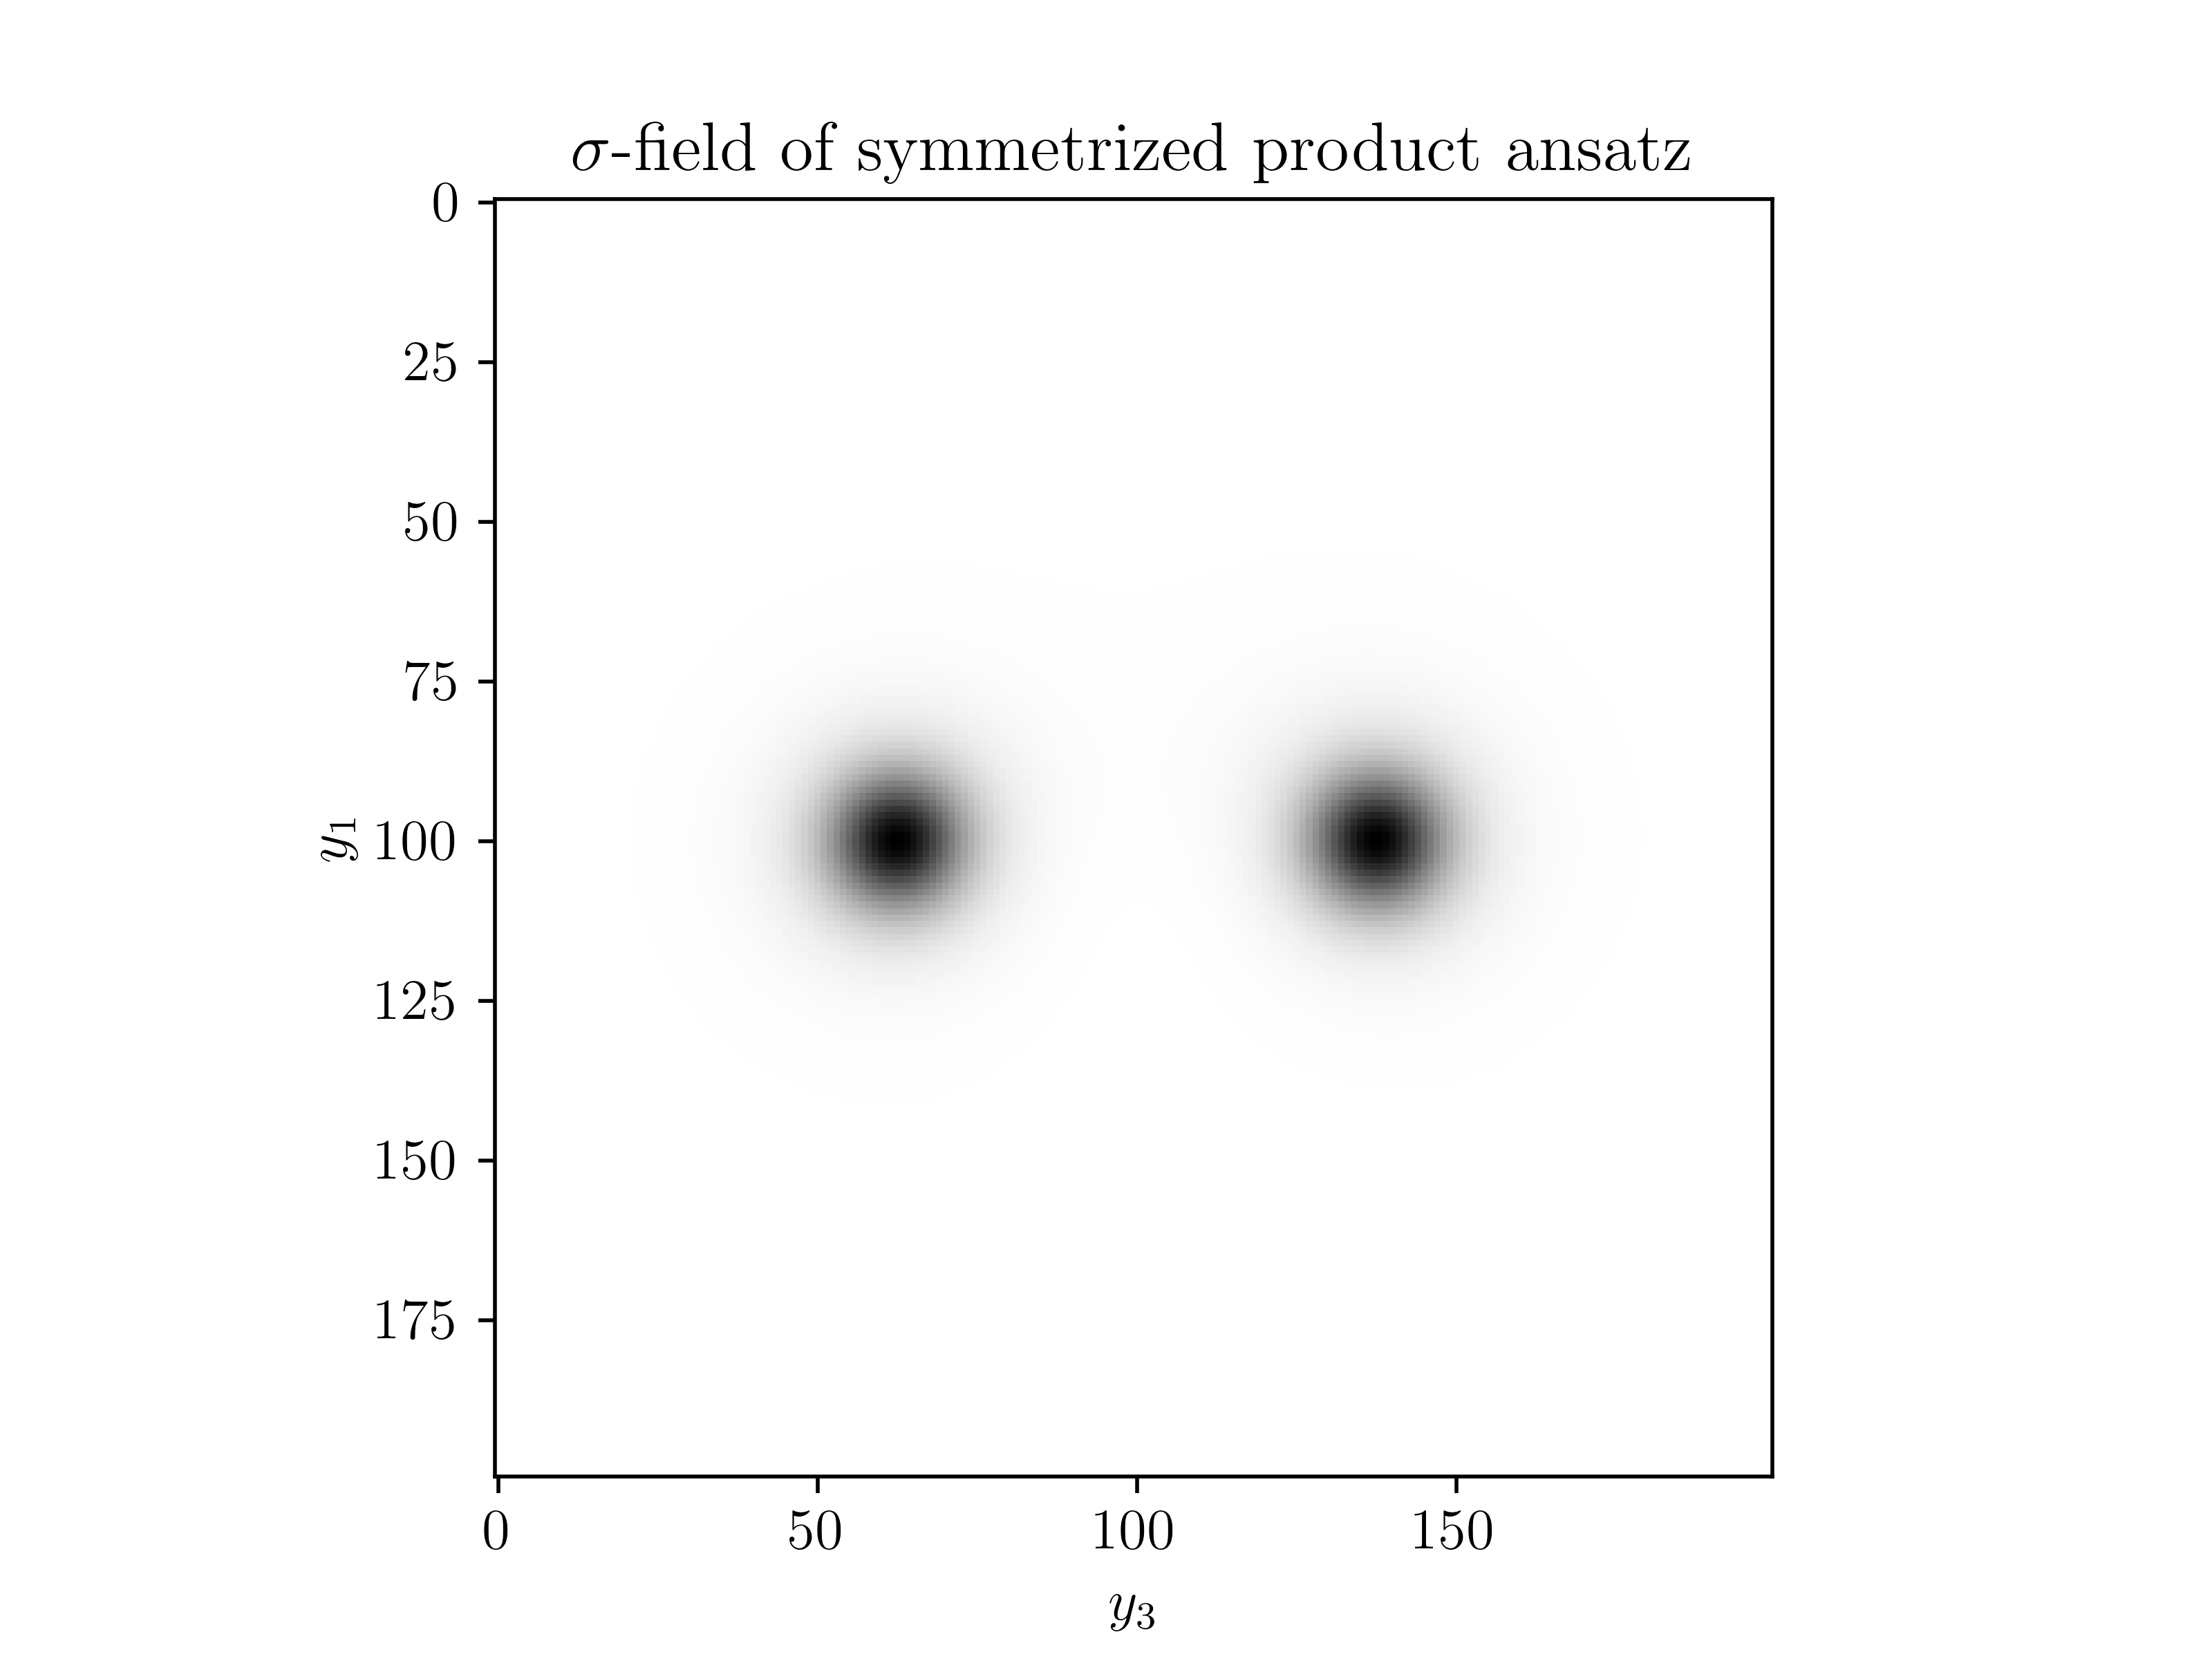
\includegraphics[width=0.8\linewidth]{./revistas/001/imaxes/fig1.png}
    \caption{Figura 1}
    \label{fig:figura1}
\end{figure}

\subsection*{Cadros} %%%%%%%%%%%%%%%%%%%%%%%%%%%%%%%%%%%%%%%%%%%%%%%%%%%%%%%%

Pódense facer cadros moi simples pero que eu creo que quedan moi ben sen ter que recurrir a páxinas externas:

\begin{table}[h!]
\centering
\begin{tabular}{cc} % número de columnas = número de c
    \toprule
    \midrule
    \multicolumn{2}{c}{información xeral ao cadro} \\ % \multicolumn{número de columnas}{aliñamento}
    \midrule
    {título de outra columna} & {título dunha columna} \\
    \midrule
    \toprule

    {11} & {12} \\
    \midrule
    {21} & {22} \\

    \midrule
    \bottomrule
\end{tabular}
\caption{Cadro 1}
\label{Tab:cadro1}
\end{table}
